\documentclass[10pt,a4paper]{article}
\usepackage[utf8]{inputenc}
\usepackage[T1]{fontenc}
\usepackage{amsmath}
\usepackage{amssymb}
\usepackage{graphicx}

\newtheorem{theorem}{Theorem}
\newtheorem{definition}{Definition}
\usepackage{algorithm}
\usepackage{algpseudocode}
\usepackage{listings, lstautogobble}
\lstset{
	language=Matlab, autogobble=true
}
\title{Numerik MA0008: Zusammenfassung}
\author{Jonas Treplin}
\begin{document}
	\maketitle
	\section{Grundlagen}
	\begin{theorem}[Satz von Gerschgorin]
		Sei $(a_{ij})=A \in \mathbb{R}^{n\times n}$ dann sind die Eigenwerte von $A$ enthalten in $\bigcup_{i=1}^{n}S_i \subset \mathbb{C}$, dabei sind die $S_i := K(a_{ii}, \sum_{j=1, i\neq j}^{n})$. Wobei mindestens ein Eigenwert jeder Zusammenhangskomponente zugeordnet ist.
	\end{theorem}
	\section{Matrixfaktorisierung}
	\begin{theorem}
		Die Permutationsmatrizen, die unitären Matrizen, die invertierbaren Matrizen und die unteren/oberen Dreiecksmatrizen bilden jeweils unter Matrixmultiplikation eine Gruppe. Insbesondere sind ihre Inverse von der selben Klasse von Matrizen. 
	\end{theorem}
	Gleichungssysteme für die unitären Matrizen (und damit auch Permutationsmatrizen) lassen sich einfach durch adjungieren lösen. Für untere und obere Dreiecksmatrizen existieren Vorwärts- und Rückwärtssubsitution.  Diese sind aus dem Endschritt des Lösens von Gleichungssystemen mit dem Gauß-Algorithmus bekannt.
	\begin{algorithm}
		\caption{Vorwärtssubsitution (Lösen einer unteren Dreiecksmatrix)}
		\begin{algorithmic}
			\Require $(l_{ij}) = L \in \mathbb{R}^{n\times n}$ Untere Dreiecksmatrix, $b \in \mathbb{R}^n$.
			\For{$i\in 1:n$}
				\State $x_i \leftarrow \frac{1}{l_{ii}}(b_i - \sum_{j=1}^{i-1}l_{ij}*x_j)$
			\EndFor
		\end{algorithmic}
	\end{algorithm}
	\begin{algorithm}
		\caption{Rückwärtsssubsitution (Lösen einer oberen Dreiecksmatrix)}
		\begin{algorithmic}
			\Require $(u_{ij}) = U \in \mathbb{R}^{n\times n}$ Obere Dreiecksmatrix, $b \in \mathbb{R}^n$.
			\For{$i\in n:1$}
			\State $x_i \leftarrow \frac{1}{u_{ii}}(b_i - \sum_{j=i+1}^{n}u_{ij}*x_j)$
			\EndFor
		\end{algorithmic}
	\end{algorithm}
	Glücklicherweise kann jede invertierbare Matrix (fast eindeutig) in solche Matrizen zerlegt werden. Dies geschieht Wahlweise durch eine LU-Zerlegung oder eine QR-Zerlegung.
	\begin{algorithm}
		\caption{LU-Zerlegung ohne Pivots}
		\begin{algorithmic}
			\Require $(a_{ij}) = A \in GL(n)$
			\For{$i\in 1:n$}
				\State $l_{ii} \leftarrow 1$
				\For{$j \in i+1:n$}
					\State $l_{ji} \leftarrow -\frac{a_{ji}}{a_{ii}}$
					\For{$k\in i:n$}
						\State $u_{jk} \leftarrow u_{jk} - a_{ji}a_{ji}$
					\EndFor
				\EndFor
			\EndFor
		\end{algorithmic}
	\end{algorithm}
	Mit Pivots erreicht man, dass jede invertierbare Matrix $A \in GL(n)$ zerlegt werden kann, sodass $PA = LU$. Dazu wählt man in jedem Schritt $i$ die Zeile $j = \arg \max_{j\geq i} |a^i_{ji}|$ und vertauscht diese mit der $i$-ten Zeile. 
	\begin{theorem}[LU-ZErlegung mit Pivots]
		Sei $A \in GL(n)$. Dann existieren eine eindeutige Permutationsmatrix $P$, sowie untere (obere) Dreiecksmatrix $L$ ($U$, sodass $PA =LU$. Dabei ist $L$ normiert also $l_{ii}= 1$.
	\end{theorem}
	\begin{theorem}[Cholesky-Zerlegung]
		Sei $A$ symmetrisch positiv definit dann lässt sich eine nicht normierte untere Dreiecksmatrix $\tilde{L}$ finden, sodass $A = \tilde{L}\tilde{L}^T$.
	\end{theorem}
	\begin{algorithm}
		\caption{Berechnung der Cholesky Zerlegung}
		\begin{algorithmic}
			\Require $A$ s.p.d.
			\State $L, U \leftarrow \text{LU\_Zerlegung(A)}$
			\State $D = (u_{ii})$ Diagonalmatrix.
			\State $\tilde{L} = \sqrt{D}L$.
		\end{algorithmic}
	\end{algorithm}
	Eine weitere Möglichkeit ist die der $QR$ Zerlegung. 
	\begin{definition}[Givensrotation]
		Für ein $a \in \mathbb{R}^2$ sei $Q=\begin{bmatrix}
			c & s \\
			-s & c
		\end{bmatrix}$. Wobei $c=\frac{1}{\sqrt{1+\tau^2}}$ und $s=c\tau$ mit $\tau = \frac{v_2}{v_1}$ wenn $|v_1| \geq |v_2|$ und  $s=\frac{1}{\sqrt{1+\tau^2}}$ und $c=s\tau$ mit $\tau = \frac{v_1}{v_2}$ wenn $|v_1| < |v_2|$.
	\end{definition}
	Diese Fallunterscheidung ist so gewählt, dass $||Q||\leq 1$, damit sich Rundungsfehler nicht akkumulieren.
	\begin{theorem}[Givens-Rotation]
		Es gilt $Qa = \xi e_1$.
	\end{theorem}
	\begin{algorithm}[H]
		\caption{QR-Zerlegung mit Givens-Rotationen}
		\begin{algorithmic}
			\Require $A \in \mathbb{R}^{n\times m}$
			\State $Q \leftarrow I_n$
			\For{$i \in [n]$}
				\For{$j \in (n, ..., i+1)$}
					\State $G : = \begin{bmatrix}
					1 &  &  &  &  &  \\
					& \ddots &  &  &  &  \\
					&  & c & s &  &  \\
					&  & -s & c &  &  \\
					&  &  &  & \ddots &  \\
					&  &  &  &  & 1
				\end{bmatrix} \leftarrow Givens(\begin{bmatrix}
						A_{j-1,i} \\
						A_{j-1,i}
					\end{bmatrix})$
					\State $Q \leftarrow GQ$
					\State $A \leftarrow GA$
				\EndFor
			\EndFor
			\State $Q \leftarrow Q*$
		\end{algorithmic}
	\end{algorithm}
	\begin{definition}[Householder Spiegelung]
		Die Householder Spiegelung für einen Vektor $a \in \mathbb{R}^n$ ist:
		$$Q := Id -\frac{2}{v^Tv}vv^T$$
		Wobei $v :=a+\text{sign}(a_1)||a||e_1$
		Sie erfüllt ebenfalls $Qa = \alpha e_1$
	\end{definition}
	\begin{algorithm}
		\caption{QR-Zerlegung mit Householder Rotationen}
		\begin{algorithmic}
			\Require \Require $A \in \mathbb{R}^{n\times m}$
			\State $Q \leftarrow I_n$
			\For{$i \in [n]$}
			
			\State $H \leftarrow \begin{bmatrix}
				1 & & &    \\
				& \ddots & & \\
				& & 1 & \\
				& & & \text{Householder}((a_i, ..., a_n))
			\end{bmatrix}$
			\State $Q \leftarrow HQ$
			\State $A \leftarrow HA$
			
			\EndFor
			\State $Q \leftarrow Q*$
		\end{algorithmic}
	\end{algorithm}
	Die QR-Zerlegung ist der LU-Zerlegung hinsichtlich numerischer Stabilität überlegen, besonders bei Betrachtung der Wilkinson-Matrix:
	\begin{definition}[Wilkinson-Matrix]
		Die Wilinson-Matrix ist definiert als:
		$$W_n := \begin{bmatrix}
			1 & 0 & ... & 0 & 1\\
			-1 & \ddots & ... & \vdots & \vdots\\
			\vdots& & & \ddots & \vdots\\
			-1 & ... & ... & \dots&1
		\end{bmatrix}$$
		Ein besonders instabiler Lösungsvektor ist $b_n = \begin{bmatrix}
			0\\
			\frac{1}{n}\\
			\vdots\\
			\frac{n-2}{n}\\
			1
		\end{bmatrix}$
	\end{definition}
	\begin{figure}
		\centering
		\includegraphics{"FehlerWilkinson.png"}
		\caption{Fehler beim Lösen von $W_nx =b_n$}
	\end{figure}
	\section{Fehlerrechnung}
	\begin{definition}[Fehlermaße]
		Wir definieren für eine Tupel $T= (A_1, A_2, ..., A_n)$ mit Störung $\tilde{T}=(A_+E_1, ..., A_n+E_n)$:
		\begin{itemize}
			\item das absolute Fehlermaß:
			$$[[E]]_{abs} := \max||E_i||$$
			\item das relative Fehlermaß:
			$$[[E]]_{rel}:= \max\frac{||E_i||}{||A_i||}$$
		\end{itemize}
	\end{definition}
	\begin{definition}[Maschinenepsilon]
		Das \textbf{Maschinen-$\epsilon$} is der relative Fehler, der bei Addition und Multiplikation von SKalaren auftritt. Er liegt für IEEE double-precision bei ca. $10^{-16}$
	\end{definition}
	\begin{definition}[Kondition]
		Die Kondition einer Abbildung $f$ im Punkt $x$ ist definiert als:
		$$\kappa(f, x) = \limsup_{y\to x}\frac{[[f(y)-f(x)]]}{||y-x||}$$
		Man unterscheidet zwischen:
		\begin{itemize}
			\item \textbf{gut konditionierten} Problemen: $\kappa(f,x) ~ O(1)$
			\item \textbf{schlecht konditionierten} Problemen: $\kappa(f, x) >> 1$
			\item \textbf{schlecht gestellten} Problemen: $\kappa(f, x) = \infty$
		\end{itemize}
	\end{definition}
	\begin{theorem}
		Die Kondition einer linearen Gleichung $Ax= b$ hängt nur von $A$ ab und ist:
		$$\kappa(A) = ||A||||A^{-1}||$$
	\end{theorem}
	\section{Ausgleichsrechnung}
	\begin{definition}[Lineares Ausgleichsproblem]
		Sei $A\in \mathbb{R}^{n\times n}, b\in \mathbb{R}^n$ mit $m\leq n$. Gesucht ist $x\in \mathbb{R}^m$. Sodass $$||Ax-b||_2$$ minimiert wird. Es wird im Generellen angenommen, dass $Rang(A) = m$.
	\end{definition}
	\begin{definition}[Normalengleichung]
		Gegeben ein Ausgleichsproblem $A, b$, nennt man:
		$$A^TAx=A^Tb$$
		die Normalengleichung.
	\end{definition}
	\begin{theorem}[Lösung des Linearen Ausgleichproblems mittels Normalengleichung]
		Die Lösung der Normalengleichung ist das eindeutige gesuchte Minimum des Ausgleichsproblems.
	\end{theorem}
	\begin{algorithm}
		\caption{Lösen des Ausgleichproblems mittels Normalengleichung}
		\begin{algorithmic}
			\Require Ausgleichsproblem $A\in \mathbb{R}^{n\times m}, b\in \mathbb{R}^n$
			\State $L \leftarrow$ Cholesky$(A^TA)$
			\State Löse $LL^Tx = A^Tb$ durch Vorwärts und Rückwärtsssubsitution.
		\end{algorithmic}
	\end{algorithm}
	Die Stabilität des Algorithmus hängt von der Stabilität der Matrixmultiplikation $A^TA$ ab. 
	Falls $\kappa(A^TA)$ groß ist und $||Ax-b||$ klein treten hier Stabilitätsprobleme auf. Um diesen entgegen zu wirken, kann man die Orthogonalisierungsmethode verwenden.
	\begin{algorithm}
		\caption{Lösen des Ausgleichproblems mittels QR-Methode}
		\begin{algorithmic}
			\Require Ausgleichsproblem $A\in \mathbb{R}^{n\times m}, b\in \mathbb{R}^n$
			\State Zerlege $A= Q\hat{R}$ mit $\hat{R} = \begin{bmatrix}
				R\\
				0
			\end{bmatrix}$ wobei $R\in \mathbb{R}^{m\times m}$ obere Dreiecksmatrix sei.
			\State Löse $Rx = (Q^Tb)_1$ wobei $(.)_1$ die ersten $m$ Elemente seien.
		\end{algorithmic}
	\end{algorithm}
	\begin{theorem}[Aufwand der Lösungsmethoden]
		Der Aufwand beträgt:
		\begin{enumerate}
			\item Normalengleichung: $nm^2 + \frac{m^3}{3}$.
			\item QR-Methode: $2nm^2-2\frac{m^3}{3}$
		\end{enumerate}
		Für $n >> m$ ist also die QR-Methode doppelt so teuer wie der Ansatz der Normalengleichung. 
	\end{theorem}
	\begin{theorem}[Kondition der Normalengleichung]
		Sei $A \in \mathbb{R}^{n\times m}$ und $R$ wie in der Zerlegung für die QR-Methode. Es gilt:
		$$\kappa(A^TA) = \kappa(R)^2$$
	\end{theorem}
	\section{Eigenwertapproximation}
	Eine Einfache Idee um einen einzelnen Eigenwert mit Eigenwert einer Matrix $A\in \mathbb{R}^{n\times n}$ zu bestimmen, ist die Vektoriteration. Diese beruht darauf, dass Eigenräume hoffentlich anziehende Fixpunkte sind.
	\begin{algorithm}
		\caption{Vektoriteration}
		\begin{algorithmic}
			\Require $A\in \mathbb{R}^{n\times n}$ und Startvektor $x^{(0)}\in \mathbb{R}^n$.
			\For{$i=1,2,3,...$}
				\State $y^{(i)} \leftarrow Ax^{(i-1)}$
				\State $\lambda^(i-1) \leftarrow (x^(i-1))^Ty^{(i)}$
				\State $x^{(i)} \leftarrow \frac{y^{(i)}}{||y^{(i)}||}$
			\EndFor
		\end{algorithmic}
	\end{algorithm}
	\begin{theorem}[Konvergenz der Vektoriteration]
		Sei $A\in \mathbb{R}^{n \times n}$ mit EW $|\lambda_n| \leq ... \leq |\lambda_2| < |\lambda_1|$ und EV $(v_i)_{i\in [n]}$. Dann gilt:
		$$|\lambda^{(i)}-\lambda_1| \leq C_1(x^{(0)})\vert\frac{\lambda_2}{\lambda_1}\vert^{2i}$$
		$$\Vert\text{sign}(\lambda_1)^ix^{(i)} - \text{sign}(\beta_1)v_1\Vert_2 \leq C_2(x^{(0)})|\frac{\lambda_2}{\lambda_1}|^i$$
		Wobei $\beta_1 := v^T_1x^{(0)}$ und $C_1, C_2$ Konstanten sind die vom Startwertabhängen
	\end{theorem}
	Durch diese Methode lässt sich nur ein einzelner Eigenvektor und auch nur der zum Betragsmäßig größten Eigenwert bestimmen. Um andere Eigenvektor zu berechnen, nutzen wir, dass der Betragsmäßig größte Eignewert von $(A-\mu I)^{-1}$ der Kerwehrt des nächsten Egenwerts an $\mu$ ist.
	\begin{algorithm}[H]
		\caption{Inverse Vektoriteration}
		\begin{algorithmic}
			\Require $A\in \mathbb{R}^{n\times n}$ und Startvektor $x^{(0)}\in \mathbb{R}^n$, sowie shift $\mu \in \mathbb{R}$.
			\For{$i=1,2,...$}
			\State $(A-\mu I)\omega^{(i)} = x^{(i-1)}$
			\State $\eta \leftarrow \Vert \omega^{(i)}\Vert_2$
			\State $x^{(i)} \leftarrow \omega^{(i)}/\eta$
			\State $\rho \leftarrow {x^{(i)}}^Tx^{(i-1)}/\eta$
			\State $\lambda^{(i)} \leftarrow \mu + \rho$
			\EndFor
		\end{algorithmic}
	\end{algorithm}
	Der Aufwand hängt hier davon ab, wie oft der Shiftparameter $\mu$ neu berechnet wird, dann ist jedes Mal eine LU-Zerlegung mit $O(n^3)$ Schritten nötig. Ansonsten kostet jeder Schritt $O(n^2)$ Operation hauptsächlich für Vorwärts und Rückwärtsssubsitution. \\
	Um alle Eigenwerte gleichzeitig zu bestimmen kann iterativ eine Schur-Zerlegung berechnet werden. Dies geschieht mit der QR-Iteration.
	\begin{algorithm}[H]
		\caption{QR-Iteration ohne Shift}
		\begin{algorithmic}
			\Require $A\in \mathbb{R}^{n \times n}$
			\State $A_0 \leftarrow Q_0^TAQ_0$ mit $Q\in U(n)$.
			\For{$i=1,2,3, ...$}
			\State Bestimme $Q_iR_i = A_{i-1}$
			\State $A_{i} \leftarrow R_iQ_i$
			\EndFor
		\end{algorithmic}
	\end{algorithm}
	Der Algorithmus beruht auf der Tatsache, dass $RQ \sim A$ also die gleichen EW wie $A$ hat.
	\begin{theorem}[Konvergenz der QR-Iteration]
		Sei $A\in \mathbb{R}^n$ symmetrisch und mit EW $|\lambda_1|> |\lambda_2| > ... > |\lambda_m| > 0$. Sei $A = V\Lambda V^T$ diagonalisiert mit $V$ orthogonal. Besitzt $(Q_0^TV)^{-1}$ eine normierte LU-Zerlegung, dann gilt:
		\begin{enumerate}
			\item $\lim_{k\to \infty} |(Q_k)_{ij}| = \delta_{ij}$
			\item $\lim_{k\to \infty} |(R_k)_{ij}| = \delta_{ij}|\lambda_i|$
			\item $\lim_{k\to \infty} (A_k)_{ij} = \delta_{ij}\lambda_i$
		\end{enumerate}
	\end{theorem}
	Der Beweis kann auf schwächere Bedingungen ausgweitet werden zum Beispiel sind mehrfache Eigenwerte auch erlaubt. Häufig kann die QR-Iteration auch auf nicht-symmetrische Matrizen angewendet werden, wenn sie in diesem Fall konvergiert dann allerdings nicht mehr gegen eine Diagonal-, sondern obere Dreiecksmatrix. \\
	Der erste Schritt die Transformation mit $Q_0$ transformiert die Matrix in eine obere Hessenberg Matrix. Für eine Obere Hessenberg-Matrix ist die QR-Zerlegung in $O(n^2)$ berechenbar. Da auch ein einzelner Iterationschritt die Hessenberg Form erhält beschleunigt dies das Verfahren enorm. 
	\begin{algorithm}[H]
		\caption{Berechnung von $Q_0$}
		\begin{algorithmic}
			\Require $A\in \mathbb{R}^{n\times n}$
			\State $Q_0 \leftarrow Id$
			\For{$i=1, ..., n-1}$
			\For{$j=n, i+2$}
				\State$G : = \begin{bmatrix}
					1 &  &  &  &  &  \\
					& \ddots &  &  &  &  \\
					&  & c & s &  &  \\
					&  & -s & c &  &  \\
					&  &  &  & \ddots &  \\
					&  &  &  &  & 1
				\end{bmatrix} \leftarrow Givens(\begin{bmatrix}
						A_{j-1, i} \\
						A_{j, i}
					\end{bmatrix})$
				\State $A \leftarrow GA$
				\State $Q_0 \leftarrow GQ_0$
			\EndFor
			\EndFor
		\end{algorithmic}
	\end{algorithm}
	Weiterhin kann ein Shiftparameter eingeführt werden um das Verfahren zu beschleunigen idealerweise liegt dieser Shiftparameter möglichst nah an einem Eigenwert der Matrix $A$.
	\begin{algorithm}[H]
		\caption{QR-Iteration mit Shift}
		\begin{algorithmic}
			\Require $A\in \mathbb{R}^{n \times n}$
			\State $A_0 \leftarrow Q_0^TAQ_0$ mit $Q\in U(n)$.
			\For{$i=1,2,3, ...$}
			\State $\mu_i \leftarrow \text{Shift}(A_i)$
			\State Bestimme $Q_iR_i = A_{i-1} -\mu_i I$
			\State $A_{i} \leftarrow R_iQ_i + \mu_i I$
			\EndFor
		\end{algorithmic}
	\end{algorithm}
	Dabei können verschiedene Shiftstrategien angewandt werden:
	\begin{enumerate}
		\item \textbf{Rayleighquotienten-Shift}: $\mu_i := (A_i)_{n,n}$
		\item \textbf{Wilikinson-Shift}: Bestimme die Eigenwerte $\hat\lambda_1, \hat\lambda_2$ von $\begin{bmatrix}
			(A_i)_{n-1, n-1} & (A_i)_{n-1, n} \\
			(A_i)_{n, n-1} & (A_i)_{n, n}
		\end{bmatrix}$.
		Wähle $\mu_i = \arg\max_{\mu \in \{\hat\lambda_1, \hat{\lambda_2}\}}\|\mu -(A_i)_{n,n}|$
		\item \textbf{Random-Shift}: Wählre zufällig einen Shift aus.
	\end{enumerate}
	Der Rayleighshift produziert bei $A=\begin{bmatrix}
		0 & 1 \\
		1 & 0 
	\end{bmatrix}$ als shift $0$ und landet somit in einem Deadend. Ähnlich schlägt der WIlkinson-Shift bei $A=\begin{bmatrix}
		0 & 0 & 1\\
		1 & 0 & 0 \\
		0 & 1 & 0
	\end{bmatrix}$ fehl. In diesen Situationen kommt der Random-Shift zum Einsatz. \\
	Weiterhin kann das Verfahren beschleunigt werden, indem man, sobald $|(A_i)_{n, n-1}| \leq \text{TOL}$ nur noch mit $(A_i)_{1:m-1, 1:m-1}$ weiterrechnet. Diese Strategie heißt \textbf{Deflation}. \\
	Um aus den berechneten Eigenwerten Eigenvektoren zu erhalten, kann man für wenige Eigenwerte die Inverse Vektoriteration mit Shift verwenden. Alternativ lassen sich die aus der QR-Zerlegung berechneten $Q_i$ verwenden.
	\begin{theorem}[Eigenvektoren einer oberen Dreiecksmatrix]
		Sei $R\in \mathbb{R}^n$ obere Dreiecksmatrix. Definiere:
		$$R^{(i)} := (R)_{1:i-1,1:i-1}$$
		$$\omega := (R)_{1:i-1,i}$$
		Dann hat der $i$-te Eigenvektor von $R$ die Form:
		$$v_i = \begin{pmatrix}
			(R^{(i)})^{-1}\omega \\
			-1 \\
			0 \\
			\vdots \\
			0
		\end{pmatrix}$$ 
	\end{theorem}
	\begin{theorem}[Eigenvektoren der QR-Zerlegung]
		Seien $(Q_i)_{i\in[k]}$ die berechneten $Q_i$ einer QR-Iteration auf $A$mit $Q_0$ der Umformungsmatrix für die Hessenberg-Form. Dann ist $$A_k = Q_k^T...Q_1^TQ_0^TAQ_0Q_1...Q_k$$
		Wir definieren $\hat{Q}_k := Q_0Q_1...Q_k$. Bei genügend hohem $k$ sollte $A_k$ fast gleich einer oberen Dreiecksmatrix $\hat{R}_k$ sein. Deren Eigenvektoren lassen sich berechnen nach dem obigen Satz. Dann sind die $\hat{Q}_kv_i$ die Eigenvektoren von $A$.
	\end{theorem}
	\begin{theorem}[Kondition des Eigenwertproblems für beliebige Matrizen]
		Sei $A\in \mathbb{R}^{n\times n}$. Dann exisitiert eine Konstante  $C_A$ sodass für jede Störung $\Delta A$: 
		$$\forall \mu \in \sigma(A+\Delta A) \exists \lambda_\mu\in \sigma(A): |\mu - \lambda_\mu| \leq C_A \max \{\Vert\Delta A\vert_2, \Vert \Delta A\Vert_2^{\frac{1}{n}}\}$$
	\end{theorem}
	\begin{theorem}[Bauer-Fike, Kondition des Eigenwertproblems für diagonalisierbare Matrizen]
		Sei $A\in \mathbb{R}^{n\times n}$ reell diagonalisierbar durch $T^{-1}DT$, dann existiert für jede Störung $\Delta A$ und jedes $\mu \in \sigma(A+\Delta A)$ ein $\lambda_\mu\in \sigma(A)$ mit
		$$|\mu-\lambda_mu|\leq \Vert T\Vert_p\Vert T^{-1}\Vert_p\Vert\Delta A\Vert_p$$
		Für alle $p \in [0, \infty]$.
	\end{theorem}
	\section{Interpolation}
	\begin{definition}[Interpolation]
		Gegeben Stützpunkte $(x_1, f_1), ..., (x_n, f_n)$ finde $f$ in einer bestimmten Klasse von Funktionen, sodass $f(x_i) = f_i \ \ \forall i$ 
	\end{definition}
	Die bekanntesten Formen von Interpolation sind:
	\begin{enumerate}
		\item \textbf{Polynominterpolation}: $f\in \mathbb{P}^n$
		\item \textbf{Spline-Interpolation}: $f$ ist stückweise polynomiell und gesamt $C^l$.
		\item \textbf{Rationale Interpolation}: $f \in R_{k, l}\{\frac{\sum_{i=0}^k a_ix^i}{\sum_{i=0}^lb_ix^i}\, a_i, b_j \in \mathbb{R}\}$
		\item \textbf{Trigonometrische Interpolation}: $f \in T_n := \{b_0 + \sum_{k=1}^na_ksin(2\pi kx) +\sum_{k=1}^nb_ksin(2\pi kx) \}$
	\end{enumerate}
	\begin{definition}[Lagrange-Polynom]
		Zu den $n+1$ verschiedenen Stützstellen $x_0, ..., x_n$ sind die Lagrange-Polynome von Grad $n$ definiert als:
		$$L_i(x) := \prod_{k=0, k\neq i}^n\frac{x-x_k}{x_i-x_k}$$
	\end{definition}
	\begin{theorem}[Polynominterpolation]
		Das Interpolationspolynom $\pi_n$ zu den Stützstellen $x_0, ..., x_n$ ist eindeutig definiert als:
		$$\pi_n(x) = \sum_{i=0}^{n}f_iL_i(x)$$
	\end{theorem}
	\begin{theorem}
		Die Lagrange Polynome erfüllen die Partition der $1$:
		$$\sum_{i=0}^{n}L_i(x) = 1$$
	\end{theorem}
	\begin{definition}[Vandermonde-Matrix]
		Die Matrix $V_n\in \mathbb{R}^{n+1 \times n+1}$ mit Einträgen:
		$$(V_n)_{i, j} = x_{i-1}^{j-1}$$
		Heißt Vandermonde-Matrix zu den Stützstellen $x_0, ..., x_n$.
	\end{definition}
	\begin{theorem}
		Es gilt:
		$$\det V_n = \prod_{0 \leq i < j\leq n}(x_j-x_i)$$
	\end{theorem}
	\begin{theorem}
		Das Interpolationspolynom ist auch durch $\sum_{k=0}^{n} a_kx^k$ gegeben wobei $\begin{pmatrix}
			a_0\\
			\vdots\\
			a_n
		\end{pmatrix}=: a = V_n\begin{pmatrix}
			f_0\\
			\vdots\\
			f_n
		\end{pmatrix}$
	\end{theorem}
	\begin{definition}[Knotenpolynom]
		Zu den $n+1$ Stützstellen $x_0, ..., x_n$ definiert man das Knotenpolynom 
		$$\omega_{n+1}(x)=\prod_{i=0}^n(x-x_i)$$
	\end{definition}
	\begin{theorem}
		Falls der Interpoland $f$ aus $C^{n+1}$ kommt ist der Interpolationsfehler beschränkt durch:
		$$\Vert f-\pi_n\Vert \leq \frac{\Vert\omega_{n+1}\Vert}{(n+1)!}\Vert f^{(n+1)}\Vert$$
	\end{theorem}
	\begin{theorem}
		Es gilt für jede beliebige Wahl von Punkten:
		$$\Vert\omega\Vert \geq 2^{-n}$$
	\end{theorem}
	Bei äquidistanten Stützstellen treten beim Interpolieren von $f(x) = \frac{1}{1+25x^2}$ große Fehler in den Randbereichen auf.
	\begin{figure}
		\centering
		\caption{Interpolations Fehler für $\pi_n$}
		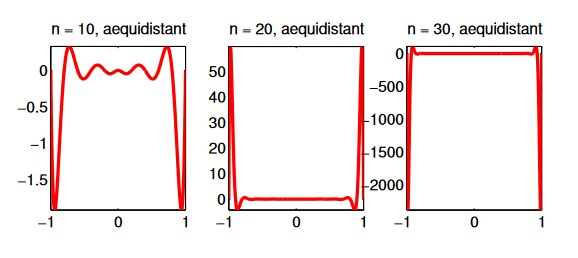
\includegraphics[scale=0.8]{rungespikes.jpg}
	\end{figure}
	Generell lässt sich keine generell optimale Knotenfolge finden. Allerdings kann $\Vert\omega_n\Vert$ minimiert werden. Dies geschieht durch die Chebychev-Punkte:
	\begin{definition}
		Die Chebychev-Polynome sind definiert als:
		$$T_n (X) := \cos(n\arccos x)$$
		Sie sind orthogonal bezüglich der Gewichtsfunktion $\frac{1}{\sqrt{1-x^2}}$. Sie besitzen die Nullstellen:
		$$x_i^{(n+1)}= \cos(\frac{2i+1}{2n+2}\pi)$$
		Diese werden auch als Chebychev-Punkte bezeichnet.
	\end{definition}
	\begin{theorem}[Dreiterm-Rekursion der Chebychev-Polynome]
		$T_0 = 1, T_1(x), T_n(x) = 2xT_{n-1}(x)-T_{n-2}(x)$
	\end{theorem}
	\begin{theorem}
		Für das Knotenpolynom $\omega_{n+1, cheb}$ zu den Chebychevpunkten gilt:
		$$\Vert\omega_{n+1,cheb} \Vert= 2^{-n}$$
	\end{theorem}
	Die theoretischen Überlegungen zur Bestimmung des Interpolationspolynom sind numerisch nicht stabil.
	\begin{algorithm}[H]
		\caption{Auswertungschema von Aitken-Neville}
		\begin{algorithmic}
			\Require $n+1$ Stützstellen $(x_0, f_0), ..., (x_n, f_n)$, Auswertungsstelle $y$.
			\State Setze $P_i(y) \leftarrow f_i$ für $i=0, ..., n$
			\For{$i=1, ..., n$}
			\For{$j=0, ..., n-i$}
			\State $P_{j...j+i}(y) \leftarrow \frac{(y-x_j)P_{j+1...j+i}(y)-(y-x_{j+i})P_{j...j+i-1}(y)}{x_{j+i}- x_{j}}$
			\EndFor
			\EndFor
		\end{algorithmic}
	\end{algorithm}
	\begin{figure}[H]
		\centering
		\caption{Darstellung des Aitken-Neville-Schema}
		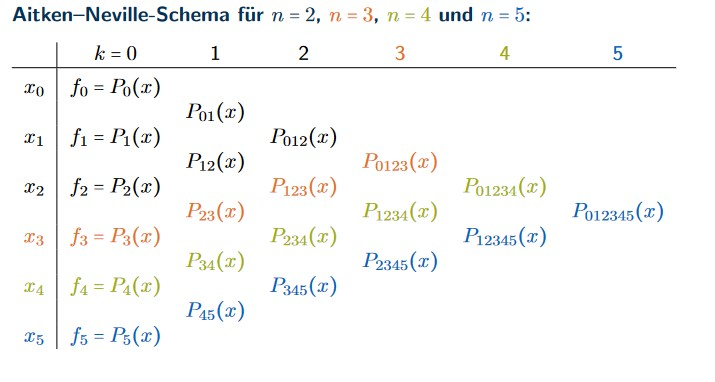
\includegraphics[scale=0.5]{aitken-neville.jpg}
	\end{figure}
	\begin{theorem}[Aufwand des Aitken-Neville-Verfahren]
		Für $l$ verschiedene Funktionen, $m$ Auswertungsstellen und $n+1$ Stützstellen beträgt der Aufwand für das Aitken-Neville-Schema $O(lmn^2)$.
	\end{theorem}
	Das Aitken-Neville Schema ist stabil aber langsam, wenn mehrere Stellen ausgwertet werden sollen. Um dies zu beschleunigen kann das 
	\begin{definition}[Newton-Darstellung eines Polynoms]
		Die Darstellung eines Polynoms in der Form:
		$$\pi_n(x) = c_0 + c_1(x-x_0) + c_2(x-x_0)(x-x_1) + ... + c_n(x-x_0)...(x-x_{n-1})$$
	\end{definition}
	\begin{algorithm}[H]
		\caption{Newton'sche Dividierte Differenzen}
		\begin{algorithmic}
			\Require $n+1$ Stützstellen $(x_0, f_0), ..., (x_n, f_n)$
			\State Setze $f[x_i]:=f_i$ für $i=0, ..., n$
			\For{$i=1, ..., n$}
			\For{$j=0, ..., n-i$}
			\State $f[x_j...x_{j+i}] \leftarrow \frac{f[x_{j+1}...x_{n-i}]-f[x_{j}...x_{n-i-1}]}{x_{j+i}- x_{j}}$
			\EndFor
			\EndFor
			\State $c_i \leftarrow f[x_0...f_i]$
		\end{algorithmic}
	\end{algorithm}
	\begin{algorithm}
		\caption{Horner-Schema}
		\begin{algorithmic}
			\Require Polynom in Newton-Darstellung mit Koeffizienten $c_0, ..., c_n$, Auswertungsstelle $y$.
			\State $p\leftarrow c_n$
			\For{$k=n-1, ..., 0$}
			\State $p \leftarrow p(y -x_k)+c_k$
			\EndFor
		\end{algorithmic}
	\end{algorithm}
	\begin{theorem}[Aufwand des Horner Schema]
		Für $l$ verschiedene Funktionen, $m$ Auswertungsstellen und $n+1$ Stützstellen beträgt der Aufwand für das Aitken-Neville-Schema $O(l(mn+n^2))$.
	\end{theorem}
	Allerdings ist das Horner-Schema \textbf{nicht stabil} für große $n$.
\end{document}